%%% Template by Mikhail Klassen, April 2013
%%% 
\documentclass[11pt,letterpaper]{article}
\newcommand{\workingDate}{\textsc{2019 $|$ April $|$ 21}}
\newcommand{\userName}{Jordan Sturtz}
\newcommand{\institution}{ Oregon State University}
\usepackage{researchdiary_png}
\usepackage{listings}
\usepackage{amsmath}

% To add your univerisity logo to the upper right, simply
% upload a file named "logo.png" using the files menu above.

\begin{document} \univlogo

\title{CS 475 - Parallel Programming}
{\Huge Project 3 Writeup}\\[5mm]

\begin{enumerate}
  \item \textbf{My Choice Quantity} 
        I added Zombie Bears to the simulation. Rather than represent these Zombie
        Bears as a quantity, however, I represented only whether the Zombie Bears
        attack. If they attack, the halve the population of deer. These Zombie 
        Bears are very picky about the weather, preferring to sleep when it
        is cold or rainy. As such, they only wake and attack 
        during when the weather exceeds 60 degrees and the precipitation is
        less than 10 inches.
    
  \item \textbf{Data} 
    \begin{lstlisting}

    Month	Precip	Temp	Height	NumDeer	ZombieBears?
    0	        8.75	20.69	1	1	
    1	        11.83	37.9	0.69	2	
    2	        10.94	37.81	7.09	1	
    3	        12.96	47.85	14.15	2	
    4	        8.52	72.63	17.11	3	
    5	        7.08	66.01	15.61	4	Attack
    6	        5.49	66.5	13.62	2	Attack
    7	        0	56.35	12.62	1	Attack
    8	        0	55.41	12.32	0	
    9	        2.16	44.47	12.6	1	
    10	        0.6	32.05	15.64	2	
    11	        4.67	26.87	16.4	3	
    12	        5.91	36.3	15.97	4	
    13	        10.19	41.8	19.88	5	
    14	        9.92	38.48	25.12	6	
    15	        12.37	51.22	29.93	7	
    16	        11.95	62.24	28.58	8	
    17	        9.09	74.74	24.63	9	
    18	        6.05	70.75	20.13	10	Attack
    19	        2.95	70.59	15.13	5	Attack
    20	        0	49.94	12.63	2	Attack
    21	        0.33	40.21	12.73	1	
    22	        2.48	31.38	15.37	2	
    23	        2.49	32.89	16.53	3	
    24	        6.21	25.07	17.78	4	
    25	        10.82	44.4	16.52	5	
    26	        10.81	53	20.57	6	
    27	        12.09	63.3	19.04	7	
    28	        10.26	60.74	15.57	8	
    29	        5.59	70.82	11.68	9	
    30	        2.52	78.44	7.18	10	Attack
    31	        1.58	73.49	2.18	5	Attack
    32	        0	48.73	0	2	Attack
    33	        0.22	36.93	0.37	1	
    34	        0.56	32.33	2.67	0	
    35	        3.96	22.72	4.49	1	
    36	        5.9	29.47	4.27	2	
    37	        8.89	39.51	5.5	3	
    38	        11.13	43.51	11.89	4	
    39	        11.69	64.2	16.87	5	
    40	        9.64	57.43	14.39	6	
    41	        8.54	74.19	11.77	7	
    42	        3.37	64.53	8.27	8	Attack
    43	        2.31	73.07	4.28	4	Attack
    44	        0	56	2.28	2	Attack
    45	        0	48.13	1.51	1	
    46	        1.69	30.82	2.53	2	
    47	        4.7	39.6	3.26	3	
    48	        6.76	29.4	7.79	4	
    49	        10.59	42.25	8.13	5	
    50	        11.06	54.62	13.21	6	
    51	        12.07	58.65	11.14	7	
    52	        9.52	55.92	7.88	8	
    53	        6.33	64.65	4.51	7	
    54	        4.59	69.44	1.03	6	Attack
    55	        2.49	60.3	0	3	Attack
    56	        0	49.05	0	1	Attack  
    57	        2.16	43.12	0.8	0	
    58	        0.6	34.56	4.73	1	
    59	        5.44	31.15	6.69	2	
    60	        9.36	24.91	8.65	3	
    61	        9.96	33.69	7.97	4	
    62	        10.42	49.08	11.34	5	
    63	        10.84	52.96	12.35	6	
    64	        8.77	64.08	10.83	7	
    65	        7.78	60.04	7.35	8	Attack
    66	        4.82	73.57	3.49	4	Attack
    67	        0.45	57.31	1.49	2	Attack
    68	        1.88	59.53	0.65	1	
    69	        0	37.76	0.24	0	
    70	        3.15	28.04	3.04	1	
    71	        4.32	38.34	3.74	2	
    72	        5.84	38.5	8.37	3	

    \end{lstlisting}

    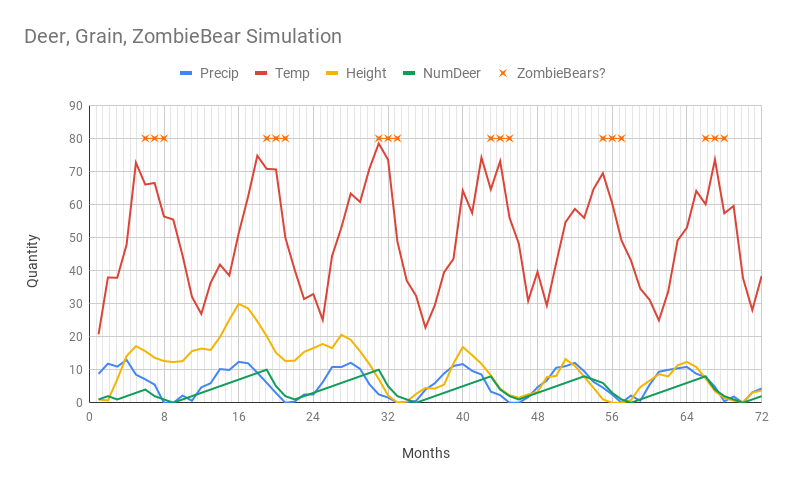
\includegraphics[width=\linewidth]{simulation}
  \item \textbf{Commentary} 

      The height of the grain, represented by the yellow line, depends on
      two key factors: first, the amount of deer, and second the weather 
      conditions. Higher deer quantities should reduce the height of the
      grain as there are more deer grazing the land. But ideal weather 
      conditions (i.e. when temperature is close to 50 and precipitation 
      is close to 6) will tend to increase the height of the grain. 
      The graph illustrates that we tend to see peaks
      in the height graph around temperatures of 50 and with 
      precipitation around 10. We notice that it tends to be the case
      that as temperature is in decline around 50, the precipitation is
      rather low. It is for this reason that we would expect the growth
      rate to be hampered, which is evident in the graph at months 8, 20, and
      32 for example. The height of the grain is also affected negatively 
      by the number of deer. We see that as the number of deer increases
      as represented by the green line, we see a decline in the grain height.

      The number of deer is affected by one of two things: whether the
      number of deer is greater than the height of the grain or whether
      the Zombie Bears attack. In cases where the Zombie Bears do not attack,
      we notice that when the height of the grain is greater than the 
      number of deer (i.e. the yellow line is greater than the green line), 
      the green line shows a steady increase by one deer per month, 
      which matches expectation.

      The orange X's in the above graph represent whether the Zombie Bears 
      attacked. As can be seen in the above data, they attack only when the
      the temperature exceeds 60 and the precipitation drops below 10. Moreover,
      For each attack, the NumDeer variable halves. In the graph we see a 
      precipitous drop in the green line for each Zombie Bear attack. 

      The temperature and precipitation are determined by a sine wave function
      with some added randomness, which matches the periodic patterns we 
      see in the red and blue lines. 

\end{enumerate}
\end{document}
